% include the figures path relative to the master file
\graphicspath{ {./content/intro/figures/} }

\section{Introduction}
\label{sec:intro}  % \label{} allows reference to this section


Breast cancer is the second most common cancer (1.4 million cases per year, 10.9\% of  diagnosed cancers) after lung cancer, followed by colorectal, stomach, prostate and liver cancers~\cite{Ferlay2010}.
In terms of mortality, breast cancer is the fifth most common cause of cancer death.
However, it place as the leading cause of cancer death among females both in western countries and in economically developing countries~\cite{cancerStatistics2011}.

Medical imaging plays an important role in breast cancer mortality reduction, contributing to its early detection through screening, diagnosis, image-guided biopsy, treatment follow-up and suchlike procedures~\cite{smith2003american}.
Although \ac{dm} remains the reference imaging modality, \ac{us} imaging has proven to be a successful adjunct image modality for breast cancer screening~\cite{smith2003american,berg2004diagnostic}, specially as a consequence of the discriminative capabilities that \ac{us} offers for differentiating between solid lesions that are benign or malignant~\cite{Stavros:1995p12392} so that the amount of unnecessary biopsies, which is estimated to be between $65\sim85\%$ of the prescribed biopsies~\cite{yuan2010multimodality}, can be reduced~\cite{ciatto1994contribution} in replacing them by short-term \ac{us} screening follow-up~\cite{gordon1995malignant}.

Figure \dots shows \dots what doctors look for. The image needs to be compacted and would be further used to justify the features used.

Analysing figre \dots it can be observed that most of the markers depend on the lesion delineation.
Therefore in order to develop releable \ac{cad} systems accurate segmentations to properly delineate the lesions are needed. 
This article presents a segmentation technique based on classifying superpixels based on their appearance.

\begin{figure}[htpb]
  \centering
  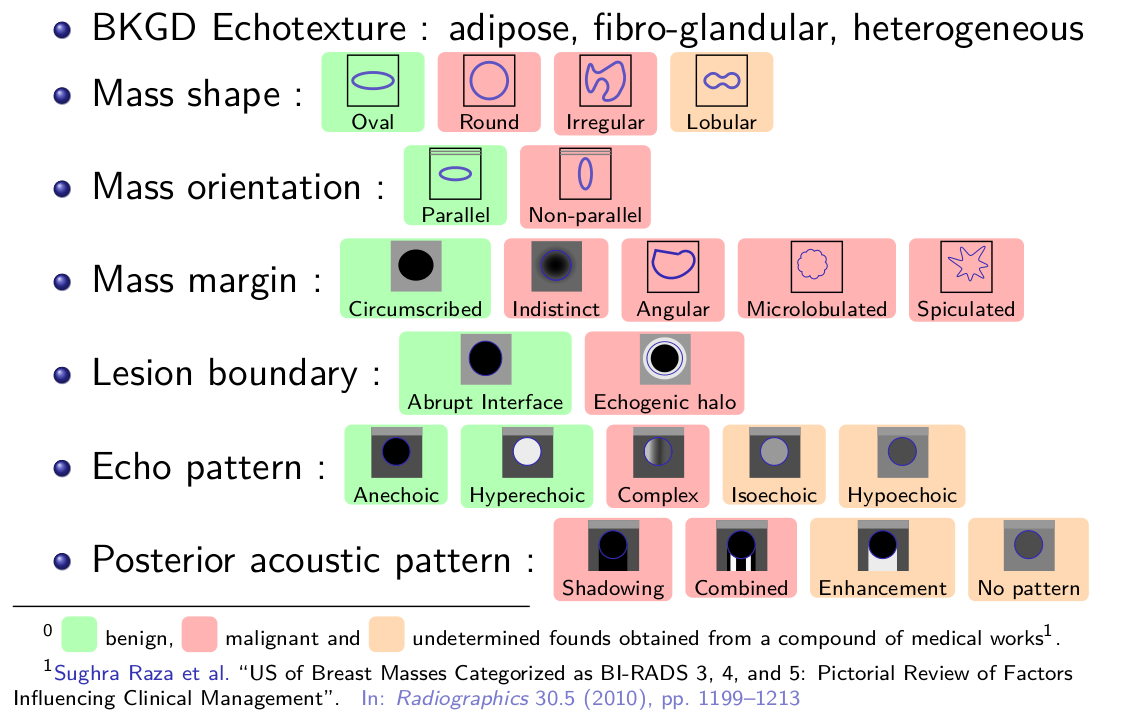
\includegraphics[width=0.9\linewidth]{doc}
  \caption{Visual compilation of breast lesions characteristics}
  \label{fig:lesions}
\end{figure}

%Regardless of the clinical utility of the \ac{us} images, such image modality suffers from different inconveniences due to strong noise natural of \ac{us} imaging  and the presence of strong \ac{us} artifacts, both degrading the overall image quality~\cite{Ensminger:2008p6920} which compromise the performance of the radiologists.
%Radiologists infer health state of the patients based on visual inspection of images which by means of some screening technique (e.g.~\ac{us}) depict physical properties of the screened body.
%The radiologic diagnosis error rates are similar to those found in any other tasks requiring human visual inspection, and such errors, are subject to the quality of the images and the ability of the reader to interpret the physical properties depicted on them\cite{manning2005perception}.
%
%Therefore the interest from the medical imaging community, also for the specific case of breast lesion assessment using \ac{us} data, in developing \ac{cad} systems that provide better instrumentation to improve image interpretation, and consequently achieve better diagnosis.

%%% Local Variables: 
%%% mode: latex
%%% TeX-master: "../../master.tex"
%%% End: \section{introduction}
